\chapter{Methodology}

\section{Adding a Figure}

%To add a figure, upload your png and use the following code: 

%%%%%%%%%%%%%%%%%%%%%%%%%%%%%%%%%%%%%%%%%%%
\begin{figure}[H]
    \centering
    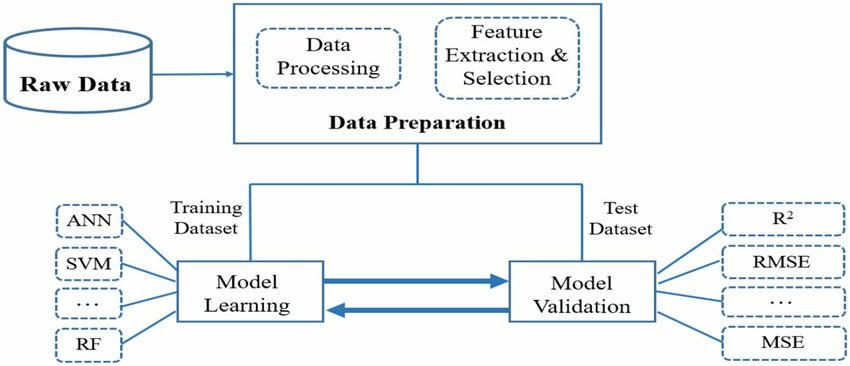
\includegraphics[width=0.8\textwidth]{Figures/Fig:ML-workflow.png}
    \caption{Machine Learning Model Development Workflow}
    \label{fig:ml-workflow}
\end{figure}
%%%%%%%%%%%%%%%%%%%%%%%%%%%%%%%%%%%%%%%%%%%

% Add your figure in "include graphic {} brackets", and you can modify the size from "width"

% Add your figure title in "caption {} brackets" 

% Add your figure label in the "label {} brackets"

% You can mention your figure in any paragraph through the label using the "hash ref" as shown below:

ML model development requires several key steps, as illustrated in Figure~\ref{fig:ml-workflow}.